% JHEP.cls available at http://jhep.cern.ch/JOURNAL/tex.html
%\RequirePackage{ifpdf}
\documentclass[12pt]{article}        % For preprint
%\documentclass[12pt,draft,nohyper]{JHEP3}    % For draft
\usepackage{jheppub} % for details on the use of the package, please
\usepackage[]{float}% see the JHEP-author-manual

\usepackage{amssymb,amsfonts,bm,dsfont}
%\usepackage{draftfil}
%\usepackage{showkeys}
%\usepackage{epsfig}
%gives names of refs and cites
%If you do not have the msbm fonts, delete the following 10 lines
\font\mybb=msbm10 at 10pt
%\font\mybb=msbm12 at 12pt

\renewcommand{\arraystretch}{1.2}

\usepackage{epsfig}
%\usepackage{amssymb}

%\newcommand{\sect}[1]{\setcounter{equation}{0}\section{#1}}
%\renewcommand{\theequation}{\arabic{section}.\arabic{equation}}
%\def\appendix{{\newpage\section*{Appendix}}\let\appendix\section%
%        {\setcounter{section}{0}
%        \gdef\thesection{\Alph{section}}}\section}


%%%%%%%%%%%%%%%%%%%%%%%%%%    My Macros    %%%%%%%%%%%%%%%%%%%%%%%%%
%%%%%%%%%%%%%%%%%%%%%%%%%%%%%%%%%%%%%%%%%%%%%%%%%%%%%%%%%%%%%%%%%%%%

\def\be{\begin{eqnarray}}
\def\ee{\end{eqnarray}}
\newcommand{\nn}{\nonumber}
\newcommand\para{\paragraph{}}
\newcommand{\ft}[2]{{\textstyle\frac{#1}{#2}}}
\newcommand{\eqn}[1]{(\ref{#1})}
\newcommand{\pl}[1]{\frac{\partial L}{\partial{#1}}}
\newcommand{\ppp}[2]{\frac{\partial {#1}}{\partial {#2}}}
\newcommand{\ph}[1]{\frac{\partial H}{\partial{#1}}}

\newcommand\balpha{\mbox{\boldmath $\alpha$}}
\newcommand\bbeta{\mbox{\boldmath $\beta$}}
\newcommand\bgamma{\mbox{\boldmath $\gamma$}}
\newcommand\bomega{\mbox{\boldmath $\omega$}}
\newcommand\blambda{\mbox{\boldmath $\lambda$}}
\newcommand\bmu{\mbox{\boldmath $\mu$}}
\newcommand\bphi{\mbox{\boldmath $\phi$}}
\newcommand\bzeta{\mbox{\boldmath $\zeta$}}
\newcommand\bsigma{\mbox{\boldmath $\sigma$}}
\newcommand\bepsilon{\mbox{\boldmath $\epsilon$}}
\newcommand\btau{\mbox{\boldmath $\tau$}}
\newcommand\beeta{\mbox{\boldmath $\eta$}}
\newcommand\btheta{\mbox{\boldmath $\theta$}}
\newcommand\valpha{\vec{\alpha}}
\newcommand\vg{\vec{g}}
\newcommand{\ra}{\rightarrow}

\def\Dslash{\,\,{\raise.15ex\hbox{/}\mkern-12mu D}}
\def\Dbarslash{\,\,{\raise.15ex\hbox{/}\mkern-12mu {\bar D}}}
\def\delslash{\,\,{\raise.15ex\hbox{/}\mkern-9mu \partial}}
\def\delbarslash{\,\,{\raise.15ex\hbox{/}\mkern-9mu {\bar\partial}}}
\def\pslash{\,\,{\raise.15ex\hbox{/}\mkern-9mu p}}
\def\calDslash{\,\,{\raise.15ex\hbox{/}\mkern-12mu {\cal D}}}
\newcommand\Bprime{B${}^\prime$}
\newcommand{\sign}{{\rm sign}}
\newcommand{\D}{{\cal D}}
\usepackage[]{braket}
\newcommand\bte{\tilde{\bf e}}
\newcommand{\NN}{{\mathbb N}}
\newcommand{\Z}{{\bf Z}}
\newcommand{\ZZ}{{\mathbb Z}}
\newcommand{\Q}{{\bf Q}}
\newcommand{\QQ}{{\mathbb Q}}
\newcommand{\R}{{\bf R}}
\newcommand{\RR}{{\mathbb R}}
\newcommand{\C}{{\bf C}}
\newcommand{\CC}{{\mathbb C}}
\newcommand{\PP}{{\mathbb P}}
\newcommand{\e}{\,{\rm e}}
\newcommand{\CP}{{\bf CP}}
\newcommand{\Tr}{{\rm Tr}}
\newcommand{\bu}{{\bf u}}
\newcommand{\bk}{{\bf k}}
\newcommand{\bx}{{\bf x}}
\def\implies{\Rightarrow}
\def\To{\longrightarrow}
\def\longlongrightarrow{\relbar\joinrel\relbar\joinrel\rightarrow}
\def\ridiculousrightarrow{\relbar\joinrel\relbar\joinrel\relbar%
\joinrel\rightarrow}

\def\underarrow#1{\mathrel{\mathop{\longrightarrow}\limits_{#1}}}
\def\onnearrow#1{\mathrel{\mathop{\nearrow}\limits^{#1}}}
\def\undernearrow#1{\mathrel{\mathop{\nearrow}\limits_{#1}}}
\def\onarrow#1{\mathrel{\mathop{\longrightarrow}\limits^{#1}}}
\def\onArrow#1{\mathrel{\mathop{\longlongrightarrow}\limits^{#1}}}
\def\OnArrow#1{\mathrel{\mathop{\ridiculousrightarrow}\limits^{#1}}}
\def\lae{\mathrel{\mathop{\smash{\lower .5 ex \hbox{$\stackrel<\sim$}}}}}
\def\lae{\mathrel{\mathop{\smash{\lower .5 ex \hbox{$\stackrel>\sim$}}}}}
\def\eqq{\stackrel?=}

\def\theequation{\thesection.\arabic{equation}}


\setlength{\parskip}{0.4em}
\setlength{\parindent}{0pt}

\usepackage[most]{tcolorbox}
\usepackage{xcolor}

% Define Nord color scheme (basic set)
\definecolor{nord0}{HTML}{2E3440} % background
\definecolor{nord1}{HTML}{3B4252} % darker background
\definecolor{nord3}{HTML}{4C566A} % comment
\definecolor{nord4}{HTML}{D8DEE9} % foreground
\definecolor{nord7}{HTML}{8FBCBB} % teal
\definecolor{nord8}{HTML}{88C0D0} % light blue
\definecolor{nord9}{HTML}{81A1C1} % blue
\definecolor{nord10}{HTML}{5E81AC} % dark blue

% Define the tcolorbox environment for definitions
\tcbset{
  mydefstyle/.style={
    colback=nord0!05!white,
    colframe=nord10,
    coltitle=white,
    %coltext=nord1,
    fonttitle=\bfseries,
    title=Definition~\thetcbcounter,
    boxrule=0.3mm,
    arc=0mm,
    top=1mm,
    bottom=1mm,
    left=1mm,
    right=1mm,
    enhanced
  }
}

\tcbset{
  mythmstyle/.style={
    colback=nord0!02!white,
    colframe=nord8,
    coltitle=white,
    %coltext=nord1,
    fonttitle=\bfseries,
    title=Theorem~\thetcbcounter,
    boxrule=0.3mm,
    arc=0mm,
    top=1mm,
    bottom=1mm,
    left=1mm,
    right=1mm,
    enhanced
  }
}

%\newtcolorbox[auto counter, number within=section]{definition}[2][]{mydefstyle,#1}
\newtcbtheorem{definition}{Definition}{mydefstyle,#1}{def}
\newtcbtheorem{theorem}{Theorem}{mythmstyle,#1}{thm}
%%%%%%%%%%%%%%%%%%%%%   NOTES START  %%%%%%%%%%%%%%%%%%%%%%%%%%%
%%%%%%%%%%%%%%%%%%%%%%%%%%%%%%%%%%%%%%%%%%%%%%%%%%%%%%%%%%%%%%%%%


%%%%%%%%%%%%%%%%%%%%%%%%%%%%%%%%%%%%%%%%%%%%%%%%%%%%%
\title{Scratchwork and Studies related to TFIM}


\author{Ahmed Saad Sabit}

\affiliation{Department of Physics and Astronomy \\ Rice University, Houston, TX}


\emailAdd{sabit@rice.edu}


\abstract{I plan (and wish) to write \textbf{three documents} related to this research problem. 
\begin{itemize}
	\item \textbf{scratchpad and studying:} on this scratchpad, where I lay the foundation for a detailed solution.
	\item \textbf{detailed solution:} this solution should lay the foundation for the research paper (hopefully) if we do end up writing. 
	\item \textbf{Original Draft for Pre-Print}. 
\end{itemize}
First of all we look at the \emph{Transverse Field Ising Model}. }



\renewcommand{\baselinestretch}{1.05}
\usepackage{hyperref}
\begin{document} 

\maketitle
\flushbottom


\section{The Transverse Field Ising Model}
For now we will work with Spin $\frac{1}{2}$ particles. The spin of the particles are represented by a ket $\ket{ \uparrow }  = \ket{1} \in \mathcal{H}, \ket{\downarrow} = \ket{0} \in \mathcal{H}$ where $\mathcal H = \mathbb C ^2$ is a Hilbert Space for spin $\frac{1}{2}$.

Let's construct a 1+1d lattice with each site labeled as $j$ ranging from $j=1$ to $j = L$. Each site $j$ of the lattice is assigned to a Hilbert Space $\mathcal H _j  = \mathbb C ^2 $. The Hilbert Space for the lattice $\mathcal H$ is defined by 
\begin{equation}
	\label{h-original}
	\mathcal H = \mathcal H_1 \otimes \mathcal H_2 \otimes \cdots \otimes \mathcal H_L = \bigotimes_{j = 1}^{L} \mathcal H_j
\end{equation}

\begin{definition}{Transverse Field Ising Model}{tfim}
	The Hamiltonian for the Transverse Field Ising Model at Critical State on a lattice $H : \mathcal H \to \mathcal H$ is defined by \[
	H	 = - \sum_{i = 1}^{L} (Z_{i-1} Z_{i} + X_{i} )
	\]
	where $Z_i, X_i$ are Pauli Matrices, in $\ket{1}, \ket{0}$ basis given by: 
	\[
	Z_i = 
	\begin{pmatrix} 1 & 0 \\ 0 &-1 \end{pmatrix}_{i\text{-th site}}  \ \ \text{and} \ \  
	X_i = 
	\begin{pmatrix} 0 & 1 \\ 1 & 0 \end{pmatrix}_{i\text{-th site}}
	\] 
	Periodic boundary condition is invoked through $Z_{L+1}, X_{L+1} = Z_1 , X_1$.
\end{definition}
Intuitively I like to think this $Z_{j-1} Z_{j}$ as the ``bond" term (between $j-1$ and $j$ site) and $X_j$ as the site term.
%
%
%
\section*{Kramers Wannier Transformation and the Problem} 
From the Seiberg et al. paper on Non-invertible symmetries \cite{lsm} using equation $2.12$ we know that the Kramers-Wannier Transformation is given by 
\begin{align} \label{kwtrans}
	X_j & \to Z_{j-1}Z_j \notag \\ 
	Z_{j-1} Z_j & \to  X_{j-1} 
\end{align}
This transformation is a automorphism. The original and transformed Hamiltonian have an isomorphism between them, so they are mathematically the same object. We term this a duality. 
\[
	H	 = - \sum_{i = 1}^{L} (Z_{i-1} Z_{i} + X_{i} ) \to - \sum_{i = 1}^{L} (X_{i-1} + Z_{i-1}Z_i ) 
\] 
So in my intuition, each ``bond" terms become ``site" terms and vice-versa. From the same paper, from the analysis after the equation we know that there is no Unitary Operator that can achieve this transformation.

\textbf{The core problem can be shaped into finding a valid method to transform between these two dualities.}

The Non-inv-lsm paper (\cite{lsm}) solves this problem through the following method
\begin{itemize}
	\item Extend the Hilbert Space by adding a site (basically extending the lattice with one new site).
	\item Introduce a Topological Defect (discussed in the paper, on how to move and fuse them).
	\item Through motion and fusion of the defects, achieve the KW Transformation. 
\end{itemize}

The issue with this process is that we define the topological defect kind of from guesstimates and scratchwork. It's not necessarily a generalized solid method.

For us, we have a Bond Algebra theorem that leads to a different route of solution. Which I think is quite general and significantly more elegant.  


\section*{Introductory Discussions on Bond Algebra}
Before we start, let me drop the first three important definition and theorem that will be very important to whatever we do later on. 



\begin{definition}
	{Von Neumann Algebra}{neumannalg}
Let $\mathcal H$ be a Hilbert Space and let $B(\mathcal H)$ denote the algebra of bounded operators on $\mathcal H$. Bounded operator $\mathcal O$ means that there exists a finite number $0\le C$ such that $| | \mathcal O v  | | \le C | | v | | $ for every vector $v \in \mathcal H$. 
\\
\
\\
If $S \subset B(\mathcal H)$ is an arbitrary set, its commutant $S' \in B(\mathcal H)$ is the sub-algebra defined by 
\[
S' = \{\mathcal O \in B(\mathcal H)  \mid \forall \mathcal R \in S, \ \mathcal O \mathcal R = \mathcal R \mathcal O \} 
\] 

A sub-algebra (as defined above) $\mathcal A$ is a Von Neumann Algebra if it satisfies
\begin{itemize}
	\item $I \in \mathcal A$
	\item $\mathcal O \in \mathcal A \implies \mathcal O ^{\dagger} \in \mathcal A$ 
	\item Equal to bycommutant $\mathcal A = \mathcal A '' $
\end{itemize}

For a set of bonds $\hat{h}_j$, the Von Neumann Algebra $\mathcal A \{\hat{h}_j\} $ is
	\[
		\mathcal A \{h_j\} = \{\hat{I} , h_j, h_j ^{\dagger}, h_j h_{j'}, h_j^\dagger h_{j'}, h_j h_{j'}^\dagger, h ^{\dagger}_j h ^{\dagger}_{j'}, \ldots\} 
	\] 
\end{definition}
This means if any operator $\mathcal O \in \mathcal A \{h_j\} $ then $\mathcal O ^{\dagger} \in \mathcal A \{h_j\} $ also. This sets up with all the Hermitian Qualities for the problem, a favorable algebra.  
\begin{definition}{Bond Algebra Definition}{bondalg}
	A bond algebra for the Hamiltonian $H$ where $H = \sum _j \lambda_j \hat{h}_j$ with bond decomposition $\{h_j\} _j $, is the \emph{Von Neumann Algebra} $\mathcal A \{h_j\} $ generated by the bonds. Here $\lambda_j$ is a complex-valued coupling constant and $\hat{h} _j$ is a bond operator found after bond decomposition. 
\end{definition}
First of all note that the $j$ in Definition \ref{def:bondalg} can be completely general. For this problem this will probably mean the ``site index" but for other problems this could be anything: from particles to point $x$ in space of a Fourier Mode. It's a suitable label for the desired problem.

Bond Decomposition means that the Hamiltonian $H$ could be broken down to different bond operators. 
\[
H = \sum_{n}^{} \lambda_n \hat{h}_n = \sum_{\Gamma}^{} \lambda'_\Gamma \hat{h}'_\Gamma
\] 
Various decompositions can lead to different bond algebras. 

\begin{theorem}
	{insane theorem}{insane}
	Let $\mathcal A_i$ be von Neumann algebras of operators on the Hilbert Spaces $\mathcal H_i$ for $i = 1,2$. If $\Phi : \mathcal A_1 \to  \mathcal A_2$ is an \emph{isomorphism} then 
	\begin{itemize}
		\item there exists a Hilbert Space $M$ 
		\item and there exists a Unitary Transformation $U : \mathcal H_1 \otimes M \to  \mathcal H_2 \otimes M$ such that
			\[
			\Phi(\mathcal O) \otimes I = 
			U \left(\mathcal O \otimes 1 \right) U ^{\dagger}
			\]
			\[
			I \in M
			\] 
			\[
			\mathcal O \in \mathcal H_1
			\] 
	\end{itemize}
\end{theorem}


\section{Dualities as Isomorphisms: How to use Bond Algebra}
\begin{definition}
	{Duality as Isomorphism}{duality}
	Two Hamiltonians $H_1$ and $H_2$ are called \emph{dual} if there is a bond algebra $A_{H_1}$ for $H_1$ isomorphic to some bond algebra $A_{H_2}$ for $H_2$, and if the isomorphism $\Phi : A_{H_1} \to A_{H_2}$ (maps $H_1$ to $H_2$). 
\end{definition}

Lets take 
\[
	H_I [h,J] (\sigma) = \sum_i (h \sigma_i ^{x} + J \sigma_i ^{z} \sigma_{i+1} ^{z}) 
\]
Consider the basic bonds
\[
	\{\sigma_i ^{z} \sigma_{i+1} \} , \{\sigma_i^{x}\} 
\] 
These two set of operators can generate a bond algebra because 
\begin{itemize}
	\item $(\sigma_i ^{z} \sigma_{i+1}^{z}) = I$ and $(\sigma_i^{x}) ^2 = I$
	\item Hermitian because Pauli Matrices
	\item Anti commutation relation between $\sigma_i^{x}$ and $\sigma_{i-1}^{z} \sigma_i^{z}$ and $\sigma_{i}^{z} \sigma_{i+1}^{z}$ but commutation with everyone else.
	\item $\sigma_i^{z} \sigma_{i+1}^{z}$ anti commutes with $\sigma_i^{x} $ and $\sigma_{i+1}^{x}$ and commutes with everyone else. Thus we have by-commute. 
\end{itemize}

From above we see that $\sigma_i^{x}$ and $\sigma_{i}^{z} \sigma_{i+1} ^{z}$ have symmetrical behavior.
%
%
%
\newpage 
\section{The Toric Code (studied \cite{herringer})} 
% 
%
%
If I've slowly re-discovered anything again - if I don't understand something right away, I should wait until I've seen calculation related to what I didn't understand earlier. 

\begin{definition}
	{Toric Code Hamiltonian}{toricH}
Consider 2D square lattice with periodic boundary condition (hence a torus) and each \emph{edge} contains a spin $1 / 2$ particle. Define the Hamiltonian
\begin{equation}
	\label{toric}
H = - \sum_v A_v - \sum_{p}^{} B_p
\end{equation}
where the first sum is over all vertices $v$ and the second some is over all faces (or we'll call plaquette) $p $. The vertex operator $A_v$ and plaquette operator $B_p$ are \emph{tensor products of Pauli operators $X = \sigma^{x}$ and $Z = \sigma^{z}$ acting on individual spins.} 
\[
	A_v = \prod_{j \in \text{star}(v)} Z_j \ \ \text{and} \ \ 
	B_p = \prod_{j \in \text{bdy}(v)} X_j
\] 
Here $\text{star}(v)$ is the set of edges adjacent to the vertex $v$ and $\text{bdy}(p)$ is the set of edges forming the boundary of the plaquette $p$. 
\end{definition}

\begin{figure}[h]
	\centering
	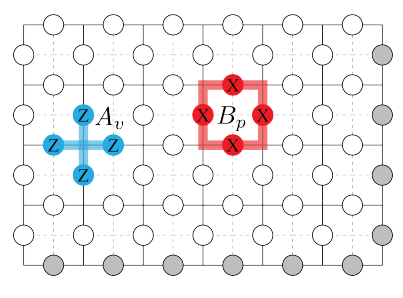
\includegraphics[width=0.5\textwidth]{./figures/toriccode.png}
	\caption{The Toric Code}
	\label{fig:-figures-toriccode-png}
\end{figure}


\textbf{On $A_v$ and $B_p$ commuting with each other}: Note that for any overlap between $A_v$ and $B_p$, the number of edges that overlap is always even. The $X $'s and $ Z$'s always anti-commute, but because there's an even number of them, they cancel out. 

Also, it's pointed out that each of the terms $A_v$ nad $B_p$ are Hermitian and square to 1. Hence the Eigenvalues are $+1, -1$. 

Because the anti-commutation effect cancels out, the ground state (or states) will be simultaneous +1 eigenstate of all the $A_v$ and $B_p$ operators. 
%
%
%
\textbf{States that satisfy above constraints}: Each square can have custody of two spin sites (``left", ``bottom" for example, and the two other sites ``right", ``top'' belong to neighbors). Each site has a Hilbert space of dimension $2$. For $N$ unit cells, there are $2N$ sites, and thus total dimension being $2^{2 N}$. 

Now, the paper requires us to think $A_v$ and $B_p$ as constraints on the Hilbert space, and violating any constraints costs energy so the ground state will obey every constraint. There's a total of $N$ number of $A_v$ and $B_p$ each. They each give $N-1$ independent constraints because the product of all $A_v$ is the identity, and similarly for $B_p$ (it also has $N-1$ constraints). 

So in total we have $2N - 2$ constraints, so we expect a Ground State Manifold of dimension $2 ^{2N - (2N - 2)} = 4$.
%
%
%
\subsection*{Ground State Construction}
\textbf{Notation}
\[\ket{0} = \ket{\uparrow} \ \ \text{and} \ \ 
\ket{1} = \ket{\downarrow}
\]
where we call $\ket{1}$ occupied and $\ket{0} $ as empty. 
So 
\[
X \ket{0} = \ket{1} \ \ \text{and} \ \ 
X \ket{1} = \ket{0}
\] 

\textbf{Study of the occupied and empty states}: Focus on $A_v$ for $v$ vertices. If a vertex $v$ has an adjacent odd number of $-1$ occupied states, then the eigenvalue of the $A_v$ for that vertex $v$ is $-1$. 

Confusingly the note is saying that $A_v$ \emph{adjacent to an occupied state is $-1$}. But I don't see how because $A_v = Z_{v, \text{down}} Z_{v, \text{right}} Z_{v, \text{top}} Z_{v, \text{left}}$. How can anything outside of these $4$ affect $A_v$?

Closed loops of occupied sites can also end up giving $+1$ eigenvalue because of coming in pairs. I should remember this from Landau's Statistical Mechanics solution of Ising model. 


Now let's introduce $B_p$. Because it's made of $X$, so it takes the plaquette and flips the states. Just by some examples its obvious that $B_p$ can create loops or deform existing loops. Another good observation is that $B_p$ cannot break or join a string of occupied edges no matter what combination of $B_p$ we use.

But here's the \textbf{topological part}. A string of occupied states that is formed across the lattice (winds around the torus) cannot be contracted into nothing, unless it has been broken. This realization gives us 4 classes of loops which cannot be deformed into one another. 
\begin{itemize}
	\item Trivial Class with no loops.
	\item A loop that winds around the torus in either directions (hence two independent class is formed).
	\item Combination of two loops with one winding around in each direction.
\end{itemize}









\newpage
\section{Dummy Introduction}


\begin{theorem}{Fluid Equation}{fluid}
\be \ppp{\rho}{t} + \nabla\cdot({\rho \bu}) = 0\ \ \ {\rm and}\ \ \  \rho\frac{D{\bf u}}{Dt} = -\nabla P\nn\ee
\end{theorem}

and using Theorem \ref{thm:fluid}


\newpage
\begin{thebibliography}{99}

\small
\parskip=0pt plus 2pt


\bibitem{son} S.~Dubovsky, L.~Hui, A.~Nicolis and D.~T.~Son,
``{\it Effective field theory for hydrodynamics: thermodynamics, and the derivative expansion},''
Phys. Rev. D \textbf{85} (2012), 085029 [arXiv:1107.0731 [hep-th]].

%\bibitem{lin} C.C. Lin, in ``{\it Liquid Helium: Proceedings of the International School of Physics ``Enrico Fermi" Course}", 1961

\bibitem{seliger} R.L. Seliger, ``{\it Variational Principles in Continuum Mechanics}", Caltech PhD Thesis 1968. 

\bibitem{lsm} Seiberg et. al. ``{\it Non-invertible Symmetries etc}", [arXiv:2401.12281]

\bibitem{poly} A.~M.~Polyakov, ``{\it Compact Gauge Fields and the Infrared Catastrophe}''
Phys. Lett. B 59 (1975), 82

\bibitem{herringer} Paul Herringer, ``{\it The Toric Code}"


\end{thebibliography}
\end{document}


%
%\begin{figure}[htb]
%\begin{center}
%\epsfxsize=3.2in\leavevmode\epsfbox{vibrator.eps}
%\end{center}
%\caption{The relative moduli space of two domain walls is a
%cigar.}
%\end{figure}
%

%
%\EPSFIGURE{openclo.eps,height=110pt}{}
%
